% commands for basic set-up
%
% Paragraph indentation:
\newcommand{\pbk}{\hspace{1.5em}}
% Unindents if needed
\newcommand{\negpbk}{\hspace*{-1.6em}}
% Gets rid of extra spacing around mathematical displays
\newcommand{\zeroout}{
    \setlength{\abovedisplayskip}{0pt}
    \setlength{\abovedisplayshortskip}{0pt}
    \setlength{\belowdisplayskip}{0pt}      
    \setlength{\belowdisplayshortskip}{0pt}
}
%
% German stuff I may want to change
%
\newcommand{\germph}[1]{\so{#1}} % German emphasis
%
% Logical/mathematical symbolism
%
% LW's N operator:
\newcommand{\nop}{\mathop{\mathrm{N}}}
% BR/LW negation:
\newcommand{\rnot}{\mathord{\sim}}
% BR/LW material implication, without and with dots:
\newcommand{\rimplies}{\supset}
\newcommand{\drimpliesd}{\mathrel{\mathord{.}\mathord{\supset}\mathord{.}}}
\newcommand{\drimplies}{\mathrel{\mathord{.}\mathord{\supset}}}
\newcommand{\ddrimpliesdd}{\mathrel{\mathord{:}\mathord{\supset}\mathord{:}}}
\newcommand{\rimpliesd}{\mathrel{\mathord{\supset}\mathord{.}}}
% BR/LW universal quantifier, with dots:
\newcommand{\ralld}[1]{\mathop{(#1)\mathord{.}}}
\newcommand{\ralldd}[1]{\mathop{(#1)\mathord{:}}}
% BR/LW existential quantifier, with and without dots:
\newcommand{\rsome}[1]{\mathop{(\mathord{\exists} #1)}}
\newcommand{\rsomed}[1]{\mathop{(\mathord{\exists} #1)\mathord{.}}}
\newcommand{\rsomedd}[1]{\mathop{(\mathord{\exists} #1)\mathord{:}}}
% Conjunction dot:
\newcommand{\rand}{\mathrel{.}}
% Disjunction with dots: 
\newcommand{\dlord}{\mathrel{\mathord{.}\mathord{\lor}\mathord{.}}}
\newcommand{\ddlordd}{\mathrel{\mathord{:}\mathord{\lor}\mathord{:}}}
% Sheffer stroke, and with dots:
\newcommand{\sheffer}{\mathrel{\vert}}
\newcommand{\dshefferd}{\mathrel{\mathord{.}\mathord{\vert}\mathord{.}}}
% Generic operator sign O'
\newcommand{\Op}{\mathop{\text{O'}}}
% Omega operators
\newcommand{\omop}[1][]{\mathop{\mathord{\Omega}^{#1}\mathord{\text{'}}}}
\newcommand{\omopparen}[2][]{\mathop{(\mathord{\Omega}^{#1})^{#2}\mathord{\text{'}}}}
% Other repeated math
\newcommand{\possibilities}{$\mathrm{K}_n = \displaystyle\sum_{\nu = 0}^{n}  \dbinom{n}{\nu}$} %4.27
\newcommand{\morepossibilities}{$\displaystyle\sum_{\kappa = 0}^{\mathrm{K}_n} \dbinom{\mathrm{K}_n}{\kappa} = \mathrm{L}_n$} %4.43
%
%
% My additions
%
\newcommand{\kckaddition}[1]{\textcolor{red}{#1}}
%
%
% Figures and drawings
%
% The cube from 5.423
\newcommand{\thecube}{\begin{center} 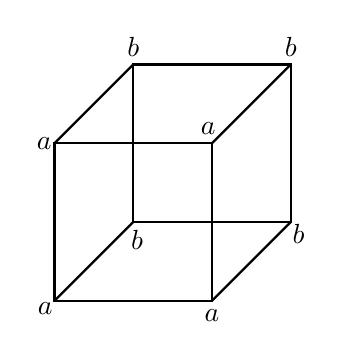
\begin{tikzpicture} [label distance=-4pt]
    \path node (aone) at (0,0) [label={[label distance=-9pt]below left:$a$}] {}
          node (atwo) at (0,2) [label={[label distance=-6pt]left:$a$}] {}
          node (athree) at (2,2) [label=above:$a\phantom{.}$] {}
          node (afour) at (2,0) [label=below:$a$] {}
          node (bone) at (1,1) [label=below:$\phantom{.}b$] {}
          node (btwo) at (1,3) [label=above:$b$] {}
          node (bthree) at (3,3) [label=above:$b$] {}
          node (bfour) at (3,1) [label={[label distance=-9pt]below right:$b$}] {};
    \draw [thick] (0,0) rectangle (2,2);
    \draw [thick] (1,1) rectangle (3,3);
    \draw [thick] (0,0) -- (1,1);
    \draw [thick] (0,2) -- (1,3);
    \draw [thick] (2,2) -- (3,3);
    \draw [thick] (2,0) -- (3,1);
 \end{tikzpicture} \end{center}}
%
% Sets German name for the eye
\newcommand{\eyename}{\textsf{Auge}}
%
% The eye from 5.6331
\newcommand{\theeye}{\eyediagram{Eye}}
\newcommand{\theauge}{\eyediagram{Auge}}
\newcommand{\eyediagram}[1]{\begin{center}
  \begin{tikzpicture}
      \path node (eye) at (0,0) [shape=circle,draw,thick,inner sep=0.05cm,label={[label distance=-3pt]left:{\textsf{#1} \thinspace---}}] {};
      \draw [thick] (-.04,0.06) arc (140:90:3cm) arc (90:-90:1cm) arc (-90:-129:3.64cm);%   
  \end{tikzpicture}   
\end{center}}
%
% Several AB-notation maps from 6.1203
\newcommand{\abfigureonegerman}{\begin{center}
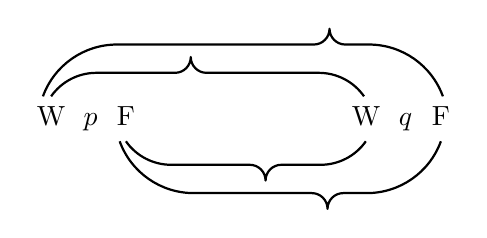
\begin{tikzpicture}[thick,line join=round]
  \node (W1) at (0,0) {\vphantom{F$pq$}W};
  \node (p) at (.5,0) {\vphantom{WF$q$}$p$};
  \node (F1) at (.95,0) {\vphantom{W$qp$}F};
  \node (W2) at (4,0) {\vphantom{F$qp$}W};
  \node (q) at (4.5,0) {\vphantom{WF$p$}$q$};
  \node (F2) at (4.95,0) {\vphantom{W$pq$}F};
  \draw (W1.110) arc (160:90:1) -- ++(2.5,0) arc 
          (-90:0:.2) arc (180:270:.2) -- ++(0.3,0) arc (90:20:1);
  \draw (W1.90) arc (145:90:.7) -- ++(1,0) arc 
          (-90:0:.2) arc (180:270:.2) -- ++ (1.427,0) arc (90:35:.7);
  \draw (F2.270) arc (-20:-90:1) -- ++(-0.3,0) arc (90:180:.2) arc (0:90:.2)
        -- ++(-1.5,0) arc (270:200:1);
  \draw (F1.270) arc (-145:-90:.7) -- ++(1,0) arc (90:0:.2) arc (180:90:.2)
    -- ++(.5,0) arc (-90:-35:.7);
\end{tikzpicture}
\end{center}}
%
\newcommand{\abfigureoneenglish}{\begin{center}
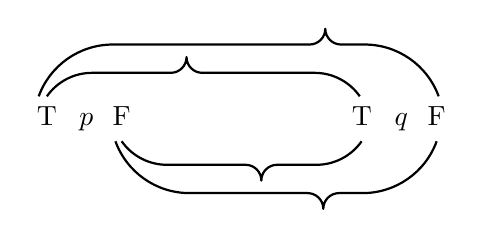
\begin{tikzpicture}[thick,line join=round]
  \node (W1) at (0,0) {\vphantom{F$pq$}T};
  \node (p) at (.5,0) {\vphantom{TF$q$}$p$};
  \node (F1) at (.95,0) {\vphantom{T$qp$}F};
  \node (W2) at (4,0) {\vphantom{F$qp$}T};
  \node (q) at (4.5,0) {\vphantom{TF$p$}$q$};
  \node (F2) at (4.95,0) {\vphantom{T$pq$}F};
  \draw (W1.110) arc (160:90:1) -- ++(2.5,0) arc 
          (-90:0:.2) arc (180:270:.2) -- ++(0.3,0) arc (90:20:1);
  \draw (W1.90) arc (145:90:.7) -- ++(1,0) arc 
          (-90:0:.2) arc (180:270:.2) -- ++ (1.427,0) arc (90:35:.7);
  \draw (F2.270) arc (-20:-90:1) -- ++(-0.3,0) arc (90:180:.2) arc (0:90:.2)
        -- ++(-1.5,0) arc (270:200:1);
  \draw (F1.270) arc (-145:-90:.7) -- ++(1,0) arc (90:0:.2) arc (180:90:.2)
    -- ++(.5,0) arc (-90:-35:.7);
\end{tikzpicture}
\end{center}}
%
%
\newcommand{\abfigureoneenglishpmc}{\begin{center}
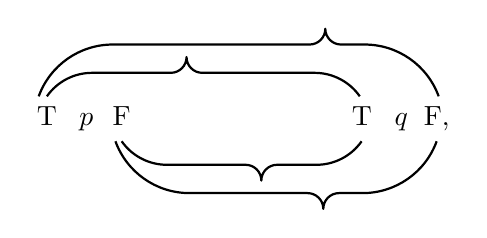
\begin{tikzpicture}[thick,line join=round]
  \node (W1) at (0,0) {\vphantom{F$pq$}T};
  \node (p) at (.5,0) {\vphantom{TF$q$}$p$};
  \node (F1) at (.95,0) {\vphantom{T$qp$}F};
  \node (W2) at (4,0) {\vphantom{F$qp$}T};
  \node (q) at (4.5,0) {\vphantom{TF$p$}$q$};
  \node (F2) at (4.95,0) {\vphantom{T$pq$}F,};
  \draw (W1.110) arc (160:90:1) -- ++(2.5,0) arc 
          (-90:0:.2) arc (180:270:.2) -- ++(0.3,0) arc (90:20:1);
  \draw (W1.90) arc (145:90:.7) -- ++(1,0) arc 
          (-90:0:.2) arc (180:270:.2) -- ++ (1.427,0) arc (90:35:.7);
  \draw (F2.270) arc (-20:-90:1) -- ++(-0.3,0) arc (90:180:.2) arc (0:90:.2)
        -- ++(-1.5,0) arc (270:200:1);
  \draw (F1.270) arc (-145:-90:.7) -- ++(1,0) arc (90:0:.2) arc (180:90:.2)
    -- ++(.5,0) arc (-90:-35:.7);
\end{tikzpicture}
\end{center}}
%
\newcommand{\abfiguretwogerman}{\begin{center}
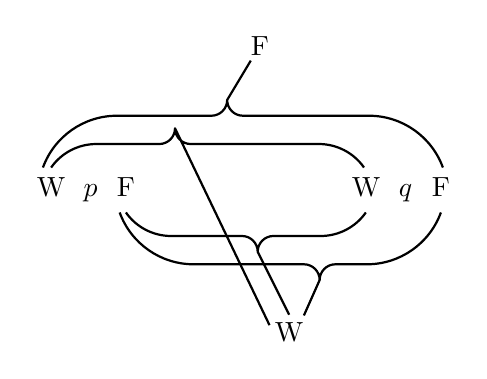
\begin{tikzpicture}[thick,line join=round]
  \node (W1) at (0,0) {\vphantom{F$pq$}W};
  \node (p) at (.5,0) {\vphantom{WF$q$}$p$};
  \node (F1) at (.95,0) {\vphantom{W$qp$}F};
  \node (W2) at (4,0) {\vphantom{F$qp$}W};
  \node (q) at (4.5,0) {\vphantom{WF$p$}$q$};
  \node (F2) at (4.95,0) {\vphantom{W$pq$}F};
  \draw (W1.110) arc (160:90:1) -- ++(1.2,0) arc (-90:0:.2) 
    -- ++(.3,.5) node [coordinate,label={[label distance=-2pt]90:~~F}] {} ++(-.3,-.5) 
    arc (180:270:.2) -- ++(1.6,0) arc (90:20:1);
  \draw (W1.90) arc (145:90:.7) -- ++(.8,0) arc (-90:0:.2) 
    -- ++(1.2,-2.5) ++(-1.2,2.5)
    arc (180:270:.2) -- ++ (1.627,0) arc (90:35:.7);
  \draw (F2.270) arc (-20:-90:1) -- ++(-0.4,0) arc (90:180:.2) 
      -- ++(-.2,-.45) ++(.2,.45)
      arc (0:90:.2)
        -- ++(-1.4,0) arc (270:200:1);
  \draw (F1.270) arc (-145:-90:.7) -- ++(0.9,0) arc (90:0:.2) 
      -- ++(.4,-.8) node [coordinate,label={[label distance=-1pt]-90:W}] {} ++(-.4,.8)   
      arc (180:90:.2)
      -- ++(.6,0) arc (-90:-35:.7);
\end{tikzpicture}
\end{center}}
%
\newcommand{\abfiguretwoenglish}{\begin{center}
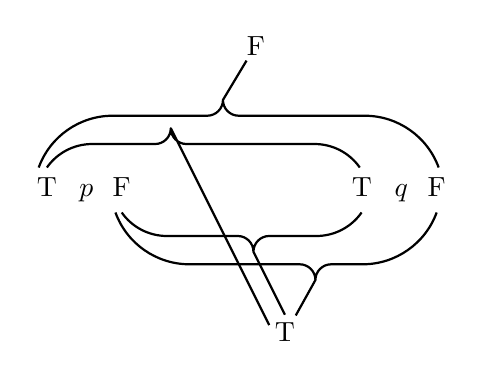
\begin{tikzpicture}[thick,line join=round]
  \node (W1) at (0,0) {\vphantom{F$pq$}T};
  \node (p) at (.5,0) {\vphantom{TF$q$}$p$};
  \node (F1) at (.95,0) {\vphantom{T$qp$}F};
  \node (W2) at (4,0) {\vphantom{F$qp$}T};
  \node (q) at (4.5,0) {\vphantom{TF$p$}$q$};
  \node (F2) at (4.95,0) {\vphantom{T$pq$}F};
  \draw (W1.110) arc (160:90:1) -- ++(1.2,0) arc (-90:0:.2) 
    -- ++(.3,.5) node [coordinate,label={[label distance=-2pt]90:~~F}] {} ++(-.3,-.5) 
    arc (180:270:.2) -- ++(1.6,0) arc (90:20:1);
  \draw (W1.90) arc (145:90:.7) -- ++(.8,0) arc (-90:0:.2) 
    -- ++(1.25,-2.5) ++(-1.25,2.5)
    arc (180:270:.2) -- ++ (1.627,0) arc (90:35:.7);
  \draw (F2.270) arc (-20:-90:1) -- ++(-0.4,0) arc (90:180:.2) 
      -- ++(-.25,-.45) ++(.25,.45)
      arc (0:90:.2)
        -- ++(-1.4,0) arc (270:200:1);
  \draw (F1.270) arc (-145:-90:.7) -- ++(0.9,0) arc (90:0:.2) 
      -- ++(.4,-.8) node [coordinate,label={[label distance=-1pt]-90:T}] {} ++(-.4,.8)   
      arc (180:90:.2)
      -- ++(.6,0) arc (-90:-35:.7);
\end{tikzpicture}
\end{center}}
%
\newcommand{\abfiguretwoenglishpmc}{\begin{center}
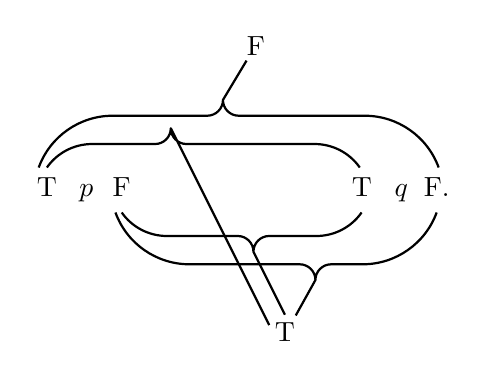
\begin{tikzpicture}[thick,line join=round]
  \node (W1) at (0,0) {\vphantom{F$pq$}T};
  \node (p) at (.5,0) {\vphantom{TF$q$}$p$};
  \node (F1) at (.95,0) {\vphantom{T$qp$}F};
  \node (W2) at (4,0) {\vphantom{F$qp$}T};
  \node (q) at (4.5,0) {\vphantom{TF$p$}$q$};
  \node (F2) at (4.95,0) {\vphantom{T$pq$}F.};
  \draw (W1.110) arc (160:90:1) -- ++(1.2,0) arc (-90:0:.2) 
    -- ++(.3,.5) node [coordinate,label={[label distance=-2pt]90:~~F}] {} ++(-.3,-.5) 
    arc (180:270:.2) -- ++(1.6,0) arc (90:20:1);
  \draw (W1.90) arc (145:90:.7) -- ++(.8,0) arc (-90:0:.2) 
    -- ++(1.25,-2.5) ++(-1.25,2.5)
    arc (180:270:.2) -- ++ (1.627,0) arc (90:35:.7);
  \draw (F2.270) arc (-20:-90:1) -- ++(-0.4,0) arc (90:180:.2) 
      -- ++(-.25,-.45) ++(.25,.45)
      arc (0:90:.2)
        -- ++(-1.4,0) arc (270:200:1);
  \draw (F1.270) arc (-145:-90:.7) -- ++(0.9,0) arc (90:0:.2) 
      -- ++(.4,-.8) node [coordinate,label={[label distance=-1pt]-90:T}] {} ++(-.4,.8)   
      arc (180:90:.2)
      -- ++(.6,0) arc (-90:-35:.7);
\end{tikzpicture}
\end{center}}
%
\newcommand{\abfigurethreegerman}{\begin{center}
\begin{tikzpicture}[thick,line join=round]
  \node (W1) at (0,0) {\vphantom{F$\xi$}„W};
  \node (xi) at (.5,0) {\vphantom{WF}$\xi$};
  \node (F1) at (.95,0) {\vphantom{W$\xi$}F{}“};
  \draw (F1.110) -- ++(-.7,.5) node [coordinate,label={[label distance=-2pt]above:W}] {};
  \draw (W1.-70) -- ++(.7,-.5) node [coordinate,label={[label distance=-2pt]below:F}] {};
\end{tikzpicture}
\end{center}}
%
\newcommand{\abfigurethreeenglish}{\begin{center}
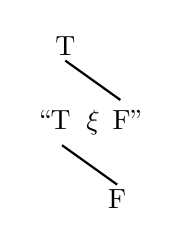
\begin{tikzpicture}[thick,line join=round]
  \node (W1) at (0,0) {\vphantom{F$\xi$}``T};
  \node (xi) at (.5,0) {\vphantom{TF}$\xi$};
  \node (F1) at (.95,0) {\vphantom{T$\xi$}F''};
  \draw (F1.110) -- ++(-.7,.5) node [coordinate,label={[label distance=-2pt]above:T}] {};
  \draw (W1.-70) -- ++(.7,-.5) node [coordinate,label={[label distance=-2pt]below:F}] {};
\end{tikzpicture}
\end{center}}
%
\newcommand{\abfigurethreeenglishpmc}{\begin{center}
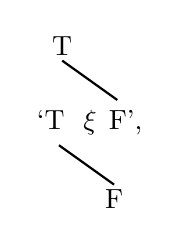
\begin{tikzpicture}[thick,line join=round]
  \node (W1) at (0,0) {\vphantom{F$\xi$}`T};
  \node (xi) at (.5,0) {\vphantom{TF}$\xi$};
  \node (F1) at (.95,0) {\vphantom{T$\xi$}F',};
  \draw (F1.110) -- ++(-.7,.5) node [coordinate,label={[label distance=-2pt]above:T}] {};
  \draw (W1.-70) -- ++(.7,-.5) node [coordinate,label={[label distance=-2pt]below:F}] {};
\end{tikzpicture}
\end{center}}
%
\newcommand{\abfigurefourgerman}{\begin{center}
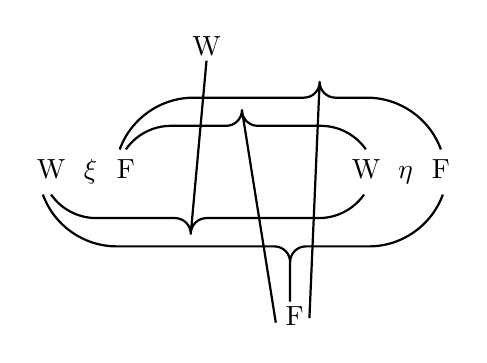
\begin{tikzpicture}[thick,line join=round]
  \node (W1) at (0,0) {\vphantom{F$\xi\eta$}W};
  \node (xi) at (.5,0) {\vphantom{WF$\eta$}$\xi$};
  \node (F1) at (.95,0) {\vphantom{W$\xi\eta$}F};
  \node (W2) at (4,0) {\vphantom{F$\xi\eta$}W};
  \node (q) at (4.5,0) {\vphantom{WF$\xi\eta$}$\eta$};
  \node (F2) at (4.95,0) {\vphantom{W$pq$}F};
   \draw (W1.-110) arc (-160:-90:1) -- ++(2,0) arc (90:0:.2) 
     -- ++(0,-.5) node [coordinate,label={[label distance=-2pt]-90:~F}] {} ++(0,.5) 
     arc (180:90:.2) -- ++(.8,0) arc (-90:-20:1);
\draw (W1.-90) arc (-145:-90:.7) -- ++(1,0) arc (90:0:.2) 
     -- ++(.2,2.2) node [coordinate,label={[label distance=-2pt]90:W}] {} ++(-.2,-2.2) 
     arc (180:90:.2) -- ++ (1.427,0) arc (-90:-35:.7);
   \draw (F2.90) arc (20:90:1) -- ++(-0.4,0) arc (-90:-180:.2) 
       -- ++(-.13,-3) ++(.13,3)
       arc (0:-90:.2)  -- ++(-1.4,0) arc (90:160:1);
   \draw (F1.90) arc (145:90:.7) -- ++(0.7,0) arc (-90:0:.2) 
       -- ++(.43,-2.7) ++(-.43,2.7)   
       arc (-180:-90:.2) -- ++(.8,0) arc (90:35:.7);
\end{tikzpicture}
\end{center}}
%
\newcommand{\abfigurefourenglish}{\begin{center}
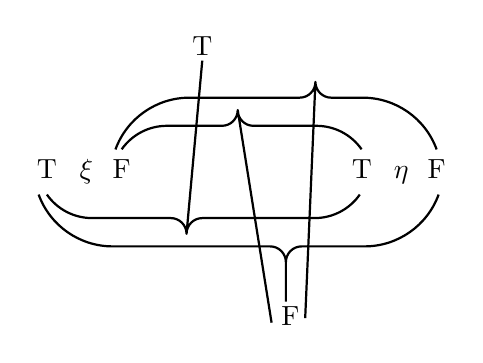
\begin{tikzpicture}[thick,line join=round]
  \node (W1) at (0,0) {\vphantom{F$\xi\eta$}T};
  \node (xi) at (.5,0) {\vphantom{TF$\eta$}$\xi$};
  \node (F1) at (.95,0) {\vphantom{T$\xi\eta$}F};
  \node (W2) at (4,0) {\vphantom{F$\xi\eta$}T};
  \node (q) at (4.5,0) {\vphantom{TF$\xi\eta$}$\eta$};
  \node (F2) at (4.95,0) {\vphantom{T$pq$}F};
   \draw (W1.-110) arc (-160:-90:1) -- ++(2,0) arc (90:0:.2) 
     -- ++(0,-.5) node [coordinate,label={[label distance=-2pt]-90:~F}] {} ++(0,.5) 
     arc (180:90:.2) -- ++(.8,0) arc (-90:-20:1);
\draw (W1.-90) arc (-145:-90:.7) -- ++(1,0) arc (90:0:.2) 
     -- ++(.2,2.2) node [coordinate,label={[label distance=-2pt]90:T}] {} ++(-.2,-2.2) 
     arc (180:90:.2) -- ++ (1.427,0) arc (-90:-35:.7);
   \draw (F2.90) arc (20:90:1) -- ++(-0.4,0) arc (-90:-180:.2) 
       -- ++(-.13,-3) ++(.13,3)
       arc (0:-90:.2)  -- ++(-1.4,0) arc (90:160:1);
   \draw (F1.90) arc (145:90:.7) -- ++(0.7,0) arc (-90:0:.2) 
       -- ++(.43,-2.7) ++(-.43,2.7)   
       arc (-180:-90:.2) -- ++(.8,0) arc (90:35:.7);
\end{tikzpicture}
\end{center}}
%
\newcommand{\abfigurefourenglishpmc}{\begin{center}
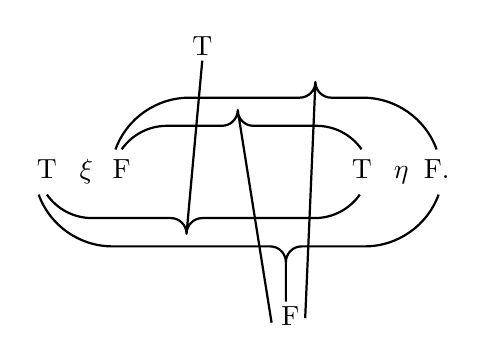
\begin{tikzpicture}[thick,line join=round]
  \node (W1) at (0,0) {\vphantom{F$\xi\eta$}T};
  \node (xi) at (.5,0) {\vphantom{TF$\eta$}$\xi$};
  \node (F1) at (.95,0) {\vphantom{T$\xi\eta$}F};
  \node (W2) at (4,0) {\vphantom{F$\xi\eta$}T};
  \node (q) at (4.5,0) {\vphantom{TF$\xi\eta$}$\eta$};
  \node (F2) at (4.95,0) {\vphantom{T$pq$}F.};
   \draw (W1.-110) arc (-160:-90:1) -- ++(2,0) arc (90:0:.2) 
     -- ++(0,-.5) node [coordinate,label={[label distance=-2pt]-90:~F}] {} ++(0,.5) 
     arc (180:90:.2) -- ++(.8,0) arc (-90:-20:1);
\draw (W1.-90) arc (-145:-90:.7) -- ++(1,0) arc (90:0:.2) 
     -- ++(.2,2.2) node [coordinate,label={[label distance=-2pt]90:T}] {} ++(-.2,-2.2) 
     arc (180:90:.2) -- ++ (1.427,0) arc (-90:-35:.7);
   \draw (F2.90) arc (20:90:1) -- ++(-0.4,0) arc (-90:-180:.2) 
       -- ++(-.13,-3) ++(.13,3)
       arc (0:-90:.2)  -- ++(-1.4,0) arc (90:160:1);
   \draw (F1.90) arc (145:90:.7) -- ++(0.7,0) arc (-90:0:.2) 
       -- ++(.43,-2.7) ++(-.43,2.7)   
       arc (-180:-90:.2) -- ++(.8,0) arc (90:35:.7);
\end{tikzpicture}
\end{center}}
%
\newcommand{\abfigurefivegerman}{
\begin{center}
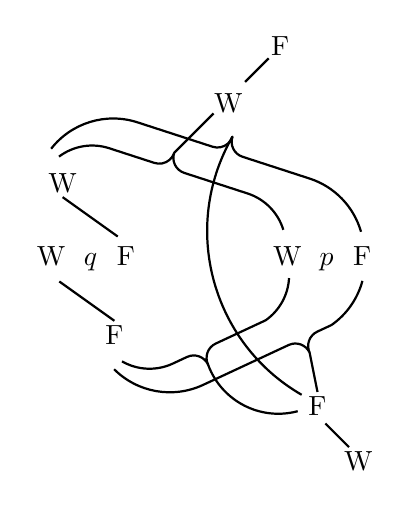
\begin{tikzpicture}[thick,line join=round]
  \node (W1) at (0,0) {\vphantom{F$pq$}W};
  \node (q) at (.5,0) {\vphantom{WF$pq$}$q$};
  \node (F1) at (.95,0) {\vphantom{W$pq$}F};
  \node (W2) at (3,0) {\vphantom{F$pq$}W};
  \node (p) at (3.5,0) {\vphantom{WF$pq$}$p$};
  \node (F2) at (3.95,0) {\vphantom{W$pq$}F};
  \draw (F1.110) -- ++(-.7,.5) node [coordinate,label={[label distance=-2pt]above:W}] {};
  \draw (W1.-70) -- ++(.7,-.5) node [coordinate,label={[label distance=-2pt]below:F}] {};
  \draw (.1,1.3) arc (127:72:0.7) -- ++(-18:0.6) arc (-109:-18:0.2) 
     -- ++(.5,.5) node (top) [coordinate,label={[label distance=-5pt]45:W}] {} ++(-.5,-.5) 
    arc (161:251:0.2) -- ++(-18:0.85) arc (72:17:0.7);
  \draw (0,1.4) arc (142:72:1) --+(-18:1) arc (-109:-18:0.2) 
    node (botone) [coordinate] {}
    arc (161:251:0.2) --+(-18:.9) arc (72:16:1);
  \draw (.9,-1.3) arc (-120:-65:.7)-- ++(25:0.2) arc (115:25:0.2) 
    node (bottwo) [coordinate] {}
    arc (-155:-245:0.2) -- ++(25:0.7) arc (-55:-3:0.7);
  \draw (.8,-1.4) arc (-135:-65:1) -- ++(25:1.2) arc (115:25:0.2) 
    -- ++(0.1,-0.5) node (bot) [coordinate,label={[label distance=-2pt]-90:F}] {} ++(-0.1,0.5)
    arc (-155:-245:0.2) -- ++(25:0.2) arc (-55:-15:1);
  \draw (top.45) ++(0.4,0.4) -- ++(0.3,0.3) node [coordinate,label={[label distance=-4pt]45:F}] {};
  \draw (botone) arc (150:240:2.4);
  \draw (bottwo) arc (-160:-75:0.95);
  \draw (bot.-45) ++ (0.1,-0.4) -- ++(0.3,-0.3) node [coordinate,label={[label distance=-2pt]-90:~~W}] {};
\end{tikzpicture}
\end{center}}
%
\newcommand{\abfigurefiveenglish}{\begin{center}
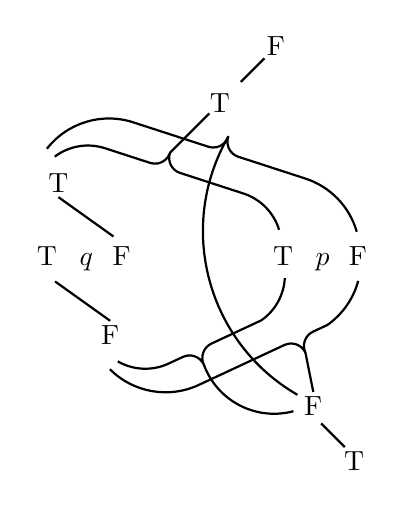
\begin{tikzpicture}[thick,line join=round]
  \node (W1) at (0,0) {\vphantom{F$pq$}T};
  \node (q) at (.5,0) {\vphantom{TF$pq$}$q$};
  \node (F1) at (.95,0) {\vphantom{T$pq$}F};
  \node (W2) at (3,0) {\vphantom{F$pq$}T};
  \node (p) at (3.5,0) {\vphantom{TF$pq$}$p$};
  \node (F2) at (3.95,0) {\vphantom{W$pq$}F};
  \draw (F1.110) -- ++(-.7,.5) node [coordinate,label={[label distance=-2pt]above:T}] {};
  \draw (W1.-70) -- ++(.7,-.5) node [coordinate,label={[label distance=-2pt]below:F}] {};
  \draw (.1,1.3) arc (127:72:0.7) -- ++(-18:0.6) arc (-109:-18:0.2) 
     -- ++(.5,.5) node (top) [coordinate,label={[label distance=-5pt]45:T}] {} ++(-.5,-.5) 
    arc (161:251:0.2) -- ++(-18:0.85) arc (72:17:0.7);
  \draw (0,1.4) arc (142:72:1) --+(-18:1) arc (-109:-18:0.2) 
    node (botone) [coordinate] {}
    arc (161:251:0.2) --+(-18:.9) arc (72:16:1);
  \draw (.9,-1.3) arc (-120:-65:.7)-- ++(25:0.2) arc (115:25:0.2) 
    node (bottwo) [coordinate] {}
    arc (-155:-245:0.2) -- ++(25:0.7) arc (-55:-3:0.7);
  \draw (.8,-1.4) arc (-135:-65:1) -- ++(25:1.2) arc (115:25:0.2) 
    -- ++(0.1,-0.5) node (bot) [coordinate,label={[label distance=-2pt]-90:F}] {} ++(-0.1,0.5)
    arc (-155:-245:0.2) -- ++(25:0.2) arc (-55:-15:1);
  \draw (top.45) ++(0.4,0.4) -- ++(0.3,0.3) node [coordinate,label={[label distance=-4pt]45:F}] {};
  \draw (botone) arc (150:240:2.4);
  \draw (bottwo) arc (-160:-75:0.95);
  \draw (bot.-45) ++ (0.1,-0.4) -- ++(0.3,-0.3) node [coordinate,label={[label distance=-2pt]-90:~~T}] {};
\end{tikzpicture}
\end{center}}
%
\newcommand{\abfigurefiveenglishpmc}{\begin{center}
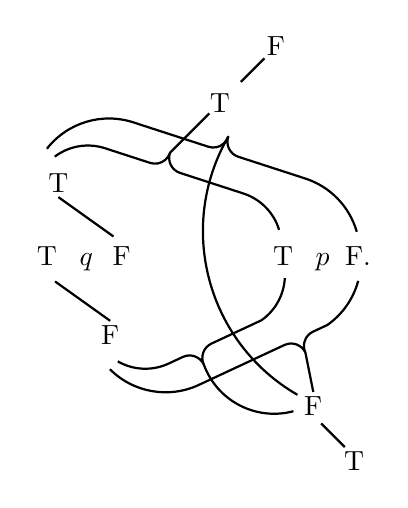
\begin{tikzpicture}[thick,line join=round]
  \node (W1) at (0,0) {\vphantom{F$pq$}T};
  \node (q) at (.5,0) {\vphantom{TF$pq$}$q$};
  \node (F1) at (.95,0) {\vphantom{T$pq$}F};
  \node (W2) at (3,0) {\vphantom{F$pq$}T};
  \node (p) at (3.5,0) {\vphantom{TF$pq$}$p$};
  \node (F2) at (3.95,0) {\vphantom{W$pq$}F.};
  \draw (F1.110) -- ++(-.7,.5) node [coordinate,label={[label distance=-2pt]above:T}] {};
  \draw (W1.-70) -- ++(.7,-.5) node [coordinate,label={[label distance=-2pt]below:F}] {};
  \draw (.1,1.3) arc (127:72:0.7) -- ++(-18:0.6) arc (-109:-18:0.2) 
     -- ++(.5,.5) node (top) [coordinate,label={[label distance=-5pt]45:T}] {} ++(-.5,-.5) 
    arc (161:251:0.2) -- ++(-18:0.85) arc (72:17:0.7);
  \draw (0,1.4) arc (142:72:1) --+(-18:1) arc (-109:-18:0.2) 
    node (botone) [coordinate] {}
    arc (161:251:0.2) --+(-18:.9) arc (72:16:1);
  \draw (.9,-1.3) arc (-120:-65:.7)-- ++(25:0.2) arc (115:25:0.2) 
    node (bottwo) [coordinate] {}
    arc (-155:-245:0.2) -- ++(25:0.7) arc (-55:-3:0.7);
  \draw (.8,-1.4) arc (-135:-65:1) -- ++(25:1.2) arc (115:25:0.2) 
    -- ++(0.1,-0.5) node (bot) [coordinate,label={[label distance=-2pt]-90:F}] {} ++(-0.1,0.5)
    arc (-155:-245:0.2) -- ++(25:0.2) arc (-55:-15:1);
  \draw (top.45) ++(0.4,0.4) -- ++(0.3,0.3) node [coordinate,label={[label distance=-4pt]45:F}] {};
  \draw (botone) arc (150:240:2.4);
  \draw (bottwo) arc (-160:-75:0.95);
  \draw (bot.-45) ++ (0.1,-0.4) -- ++(0.3,-0.3) node [coordinate,label={[label distance=-2pt]-90:~~T}] {};
\end{tikzpicture}
\end{center}}
%
\newcommand{\theline}{%
\begin{center}%
   \begin{tikzpicture}
      \draw[thick,dashed] (0.4,0) to (1,0);
      \draw[thick, o-, shorten >=3pt] (1,0) to node [below] {\scriptsize $~a$} (2,0) node {$\times$};
      \draw[thick,dashed, shorten <=3pt, shorten >=3pt] (2,0) to (2.55,0) node {$\times$};
      \draw[thick, shorten <=3pt,-o] (2.55,0) to node [below] {\scriptsize $b$} (3.55,0);% > this comment helps php syntax highlighting
      \draw[thick,dashed] (3.65,0) to (4.25,0);
   \end{tikzpicture}%
\end{center}}
%
\newcommand{\fourthreeonetablegerman}{%
\begin{tabular}{c|c|c}
$p$ & $q$ & $r$ \\ \hhline{=|=|=}
W & W & W \\ \hline%\hhline{-|-|-~-|-~-}
F & W & W \\ \hline%\hhline{-|-|-~-|-~-}
W & F & W \\ \hline%\hhline{-|-|-~-|-~~}
W & W & F \\ \hline%\hhline{-|-|-~-|-~~}
F & F & W \\ \hline%\hhline{-|-|-~~~~~}
F & W & F \\ \hline%\hhline{-|-|-~~~~~}
W & F & F \\ \hline%\hhline{-|-|-~~~~~}
F & F & F \\ \hline%\hhline{-|-|-~~~~~}
\end{tabular}\qquad
\begin{tabular}{c|c}
$p$ & $q$ \\ \hhline{=|=}
W & W \\ \hline
F & W \\ \hline
W & F \\ \hline
F & F \\ \hline   
\end{tabular}\qquad
\begin{tabular}{c}
   $p$ \\ \hhline{=}
W \\ \hline
F \\ \hline
\end{tabular}%
}
%
\newcommand{\fourthreeonetableenglish}{%
\begin{tabular}{c|c|c}
$p$ & $q$ & $r$ \\ \hhline{=|=|=}
T & T & T \\ \hline%\hhline{-|-|-~-|-~-}
F & T & T \\ \hline%\hhline{-|-|-~-|-~-}
T & F & T \\ \hline%\hhline{-|-|-~-|-~~}
T & T & F \\ \hline%\hhline{-|-|-~-|-~~}
F & F & T \\ \hline%\hhline{-|-|-~~~~~}
F & T & F \\ \hline%\hhline{-|-|-~~~~~}
T & F & F \\ \hline%\hhline{-|-|-~~~~~}
F & F & F \\ \hline%\hhline{-|-|-~~~~~}
\end{tabular}\qquad
\begin{tabular}{c|c}
$p$ & $q$ \\ \hhline{=|=}
T & T \\ \hline
F & T \\ \hline
T & F \\ \hline
F & F \\ \hline   
\end{tabular}\qquad
\begin{tabular}{c}
   $p$ \\ \hhline{=}
T \\ \hline
F \\ \hline
\end{tabular}}
%
%
\newcommand{\fourfourfourtwotablegerman}{%
{\hfil \begin{tabular}{r c|c|c l}
&$p$ & $q$ & & “ \\ \hhline{~=|=|=~}
& W  &  W  &  W &\\ \hhline{~---~}
& F  &  W  &  W &\\ \hhline{~---~}
& W  &  F  &  & \\ \hhline{~---~}
„ & F  &  F  &  W \\ \hhline{~---~}
\end{tabular} \hfil}}
%
\newcommand{\fourfourfourtwotableogden}{%
{\hfil\begin{tabular}{r c|c|c l}
`` &$p$ & $q$ & & \\ \hhline{~=|=|=~}
& T  &  T  &  T &\\ \hhline{~---~}
& F  &  T  &  T &\\ \hhline{~---~}
& T  &  F  &  & \\ \hhline{~---~}
& F  &  F  &  T & ''\\ \hhline{~---~}
\end{tabular}\hfil}
}
%
\newcommand{\fourfourfourtwotablepmc}{%
\pbk\pbk{\hfil\begin{tabular}{r c|c|c l}
` &$p$ & $q$ & & ' \\ \hhline{~=|=|=~}
& T  &  T  &  T &\\ \hhline{~---~}
& F  &  T  &  T &\\ \hhline{~---~}
& T  &  F  &  & \\ \hhline{~---~}
& F  &  F  &  T & \\ \hhline{~---~}
\end{tabular}\hfil}
}
%
\newcommand{\fiveonezeroonetablegerman}{\begin{scriptsize}\begin{tabular}{@{}l@{} @{}c@{} @{}c@{} @{}r@{} @{\thinspace}l@{~} @{~}l@{} @{~}l@{}}%
\vspace*{0pt}(W&W&W&W) & $(p,q)$ &Tautologie                  &(Wenn $p$, so $p$; und wenn $q$, so $q$.) \\
\vspace*{0pt}  & & &   &         &                             &\qquad $(p \rimplies p \rand q \rimplies q)$\\
\vspace*{0pt}(F&W&W&W) & $(p,q)$ &in Worten:                   &Nicht beides $p$ und $q$. \quad$(\rnot (p \rand q))$\\
\vspace*{0pt}(W&F&W&W) & $(p,q)$ & \phantom{i}'' \quad\quad'' &Wenn $q$, so $p$. \quad$(q \rimplies p)$\\
\vspace*{0pt}(W&W&F&W) & $(p,q)$ & \phantom{i}'' \quad\quad'' &Wenn $p$, so $q$. \quad$(p \rimplies q)$\\
\vspace*{0pt}(W&W&W&F) & $(p,q)$ & \phantom{i}'' \quad\quad'' &$p$ oder $q$. \quad$(p \lor q)$\\
\vspace*{0pt}(F&F&W&W) & $(p,q)$ & \phantom{i}'' \quad\quad'' &Nicht $q$. \quad$(\rnot q)$\\
\vspace*{0pt}(F&W&F&W) & $(p,q)$ & \phantom{i}'' \quad\quad'' &Nicht $p$. \quad$(\rnot p)$\\
\vspace*{0pt}(F&W&W&F) & $(p,q)$ & \phantom{i}'' \quad\quad'' &$p$, oder $q$, aber nicht beide. \\
\vspace*{0pt}  & & &   &         &                            &  \qquad$(p \rand \rnot q \ddlordd q \rand \rnot p)$\\
\vspace*{0pt}(W&F&F&W) & $(p,q)$ & \phantom{i}'' \quad\quad'' & Wenn $p$, so $q$; und wenn $q$, so $p$. \\
\vspace*{0pt}  & & &   &         &                            & \qquad$(p \equiv q)$\\
\vspace*{0pt}(W&F&W&F) & $(p,q)$ & \phantom{i}'' \quad\quad'' &$p$ \\
\vspace*{0pt}(W&W&F&F) & $(p,q)$ & \phantom{i}'' \quad\quad'' &$q$ \\
\vspace*{0pt}(F&F&F&W) & $(p,q)$ & \phantom{i}'' \quad\quad'' &Weder $p$ noch $q$. \\
\vspace*{0pt}  & & &   &         &                            & \qquad$(\rnot p \rand \rnot q)$ oder $(p \sheffer q )$\\
\vspace*{0pt}(F&F&W&F) & $(p,q)$ & \phantom{i}'' \quad\quad'' &$p$ und nicht $q$. \quad$(p \rand \rnot q)$ \\
\vspace*{0pt}(F&W&F&F) & $(p,q)$ & \phantom{i}'' \quad\quad'' &$q$ und nicht $p$. \quad$(q \rand \rnot p)$ \\
\vspace*{0pt}(W&F&F&F) & $(p,q)$ & \phantom{i}'' \quad\quad'' &$q$ und $p$. \quad$(q \rand p)$ \\
\vspace*{0pt}(F&F&F&F) & $(p,q)$ &\multicolumn{2}{l}{\hspace*{-7pt}Kontradiktion ($p$ und nicht $p$; und} \\
\vspace*{0pt}  & & &   &         &                            & $q$ und nicht $q$.) \quad$(p \rand \rnot p \rand q \rand \rnot q)$ \\
\end{tabular}\end{scriptsize}}
%
\newcommand{\fiveonezeroonetableogden}{\begin{scriptsize}\begin{tabular}{@{}l@{} @{}c@{} @{}c@{} @{}r@{} @{\thinspace}l@{~} @{~}l@{} @{~}l@{}}%
\vspace*{0pt}(T&T&T&T) & $(p,q)$ &Tautology                  &(if $p$ then $p$; and if $q$ then $q$) \\
\vspace*{0pt}  & & &   &         &                             &\qquad $[p \rimplies p \rand q \rimplies q]$\\
\vspace*{0pt}(F&T&T&T) & $(p,q)$ &in words:                   &Not both $p$ and $q$. \quad$[\rnot (p \rand q)]$\\
\vspace*{0pt}(T&F&T&T) & $(p,q)$ & \phantom{i}'' \quad~~'' &If $q$ then $p$. \quad$[q \rimplies p]$\\
\vspace*{0pt}(T&T&F&T) & $(p,q)$ & \phantom{i}'' \quad~~'' &If $p$ then $q$. \quad$[p \rimplies q]$\\
\vspace*{0pt}(T&T&T&F) & $(p,q)$ & \phantom{i}'' \quad~~'' &$p$ or $q$. \quad$[p \lor q]$\\
\vspace*{0pt}(F&F&T&T) & $(p,q)$ & \phantom{i}'' \quad~~'' &Not $q$. \quad$[\rnot q]$\\
\vspace*{0pt}(F&T&F&T) & $(p,q)$ & \phantom{i}'' \quad~~'' &Not $p$. \quad$[\rnot p]$\\
\vspace*{0pt}(F&T&T&F) & $(p,q)$ & \phantom{i}'' \quad~~'' &$p$ or $q$, but not both. \\
\vspace*{0pt}  & & &   &         &                            &  \qquad$[p \rand \rnot q \ddlordd q \rand \rnot p]$\\
\vspace*{0pt}(T&F&F&T) & $(p,q)$ & \phantom{i}'' \quad~~'' & If $p$, then $q$; and if $q$, then $p$. \\
\vspace*{0pt}  & & &   &         &                            & \qquad$[p \equiv q]$\\
\vspace*{0pt}(T&F&T&F) & $(p,q)$ & \phantom{i}'' \quad~~'' &$p$ \\
\vspace*{0pt}(T&T&F&F) & $(p,q)$ & \phantom{i}'' \quad~~'' &$q$ \\
\vspace*{0pt}(F&F&F&T) & $(p,q)$ & \phantom{i}'' \quad~~'' &Neither $p$ nor $q$. \\
\vspace*{0pt}  & & &   &         &                            & \qquad$[\rnot p \rand \rnot q$ or $p \sheffer q]$\\
\vspace*{0pt}(F&F&T&F) & $(p,q)$ & \phantom{i}'' \quad~~'' &$p$ and not $q$. \quad$[p \rand \rnot q]$ \\
\vspace*{0pt}(F&T&F&F) & $(p,q)$ & \phantom{i}'' \quad~~'' &$q$ and not $p$. \quad$[q \rand \rnot p]$ \\
\vspace*{0pt}(T&F&F&F) & $(p,q)$ & \phantom{i}'' \quad~~'' &$p$ and $q$. \quad$[p \rand q]$ \\
\vspace*{0pt}(F&F&F&F) & $(p,q)$ &\multicolumn{2}{l}{\hspace*{-7pt}Contradiction ($p$ and not $p$; and} \\
\vspace*{0pt}  & & &   &         &                            & $q$ and not $q$.) \quad$[p \rand \rnot p \rand q \rand \rnot q]$ \\
\end{tabular}\end{scriptsize}}
%
\newcommand{\fiveonezeroonetablepmc}{\begin{scriptsize}\begin{tabular}{@{}l@{} @{}c@{} @{}c@{} @{}r@{} @{\thinspace}l@{~} @{~}l@{} @{~}l@{}}%
\vspace*{0pt}(T&T&T&T) & $(p,q)$ &Tautology                  &(If $p$ then $p$; and if $q$ then $q$.) \\
\vspace*{0pt}  & & &   &         &                             &\qquad $(p \rimplies p \rand q \rimplies q)$\\
\vspace*{0pt}(F&T&T&T) & $(p,q)$ &In words:                   &Not both $p$ and $q$. \quad$(\rnot (p \rand q))$\\
\vspace*{0pt}(T&F&T&T) & $(p,q)$ & \phantom{i}'' \quad~~''\quad: &If $q$ then $p$. \quad$(q \rimplies p)$\\
\vspace*{0pt}(T&T&F&T) & $(p,q)$ & \phantom{i}'' \quad~~''\quad: &If $p$ then $q$. \quad$(p \rimplies q)$\\
\vspace*{0pt}(T&T&T&F) & $(p,q)$ & \phantom{i}'' \quad~~''\quad: &$p$ or $q$. \quad$(p \lor q)$\\
\vspace*{0pt}(F&F&T&T) & $(p,q)$ & \phantom{i}'' \quad~~''\quad: &Not $q$. \quad$(\rnot q)$\\
\vspace*{0pt}(F&T&F&T) & $(p,q)$ & \phantom{i}'' \quad~~''\quad: &Not $p$. \quad$(\rnot p)$\\
\vspace*{0pt}(F&T&T&F) & $(p,q)$ & \phantom{i}'' \quad~~''\quad: &$p$ or $q$, but not both. \\
\vspace*{0pt}  & & &   &         &                            &  \qquad$(p \rand \rnot q \ddlordd q \rand \rnot p)$\\
\vspace*{0pt}(T&F&F&T) & $(p,q)$ & \phantom{i}'' \quad~~''\quad: & If $p$ then $q$, and if $q$ then $p$. \\
\vspace*{0pt}  & & &   &         &                            & \qquad$(p \equiv q)$\\
\vspace*{0pt}(T&F&T&F) & $(p,q)$ & \phantom{i}'' \quad~~''\quad: &$p$ \\
\vspace*{0pt}(T&T&F&F) & $(p,q)$ & \phantom{i}'' \quad~~'' &$q$ \\
\vspace*{0pt}(F&F&F&T) & $(p,q)$ & \phantom{i}'' \quad~~''\quad: &Neither $p$ nor $q$. \\
\vspace*{0pt}  & & &   &         &                            & \qquad$(\rnot p \rand \rnot q$ or $p \sheffer q)$\\
\vspace*{0pt}(F&F&T&F) & $(p,q)$ & \phantom{i}'' \quad~~''\quad: &$p$ and not $q$. \quad$(p \rand \rnot q)$ \\
\vspace*{0pt}(F&T&F&F) & $(p,q)$ & \phantom{i}'' \quad~~''\quad: &$q$ and not $p$. \quad$(q \rand \rnot p)$ \\
\vspace*{0pt}(T&F&F&F) & $(p,q)$ & \phantom{i}'' \quad~~''\quad: &$q$ and $p$. \quad$(q \rand p)$ \\
\vspace*{0pt}(F&F&F&F) & $(p,q)$ &\multicolumn{2}{l}{\hspace*{-7pt}Contradiction ($p$ and not $p$, and} \\
\vspace*{0pt}  & & &   &         &                            & $q$ and not $q$.) \quad$(p \rand \rnot p \rand q \rand \rnot q)$ \\
\end{tabular}\end{scriptsize}}
%
\newcommand{\sixzerotwostackonegerman}{\[ \begin{aligned}     &x = \omop[0] x \text{ Def.\ und} \\
     &\omop \omop[\nu] x = \omop[\nu + 1] x \text{ Def.} \end{aligned} \]}
\newcommand{\sixzerotwostackoneogden}{\[ \begin{aligned}     &x = \omop[0] x \text{ Def.\ and} \\
     &\omop \omop[\nu] x = \omop[\nu + 1] x \text{ Def.} \end{aligned} \]}
\newcommand{\sixzerotwostackonepmc}{\[ \begin{aligned}     &x = \omop[0] x \text{ Def.} \\
     &\omop \omop[\nu] x = \omop[\nu + 1] x \text{ Def.} \end{aligned} \]}
%
\newcommand{\sixzerotwostacktwogerman}{\[\begin{aligned} &0+1=1 \text{ Def.}\\
                   &0+1+1=2 \text{ Def.}\\
                   &0+1+1+1=3 \text{ Def.}\\
                   &\text{(u.\,s.\,f.)} 
    \end{aligned}\]}
\newcommand{\sixzerotwostacktwoogden}{\[ \begin{aligned} &0+1=1 \text{ Def.}\\
                   &0+1+1=2 \text{ Def.}\\
                   &0+1+1+1=3 \text{ Def.}\\
                   &\text{and so on.} 
    \end{aligned}\]}
\newcommand{\sixzerotwostacktwopmc}{\[ \begin{aligned} 0+1&=1 \text{ Def.,}\\
                   0+1+1&=2 \text{ Def.,}\\
                   0+1+1+1&=3 \text{ Def.,}\\
                   \text{(and so}&\text{ on).} 
    \end{aligned}\]}
%
\usepackage{newunicodechar,xspace}
\newunicodechar{…}{\ifmmode\dots\else\ldots\xspace\fi}
\newunicodechar{“}{\text{\textquotedblleft\xspace}}
\newunicodechar{‘}{\text{\textquoteleft\xspace}}
\xspaceaddexceptions{]\}’”}